\section{Introduction}



World models \cite{WM_Survey} are rapidly emerging as a central substrate for physical AI. Beyond recent progress in video generation, they are increasingly expected to support physical understanding, temporal prediction, embodied interaction, and, ultimately, continual adaptation in real environments. In this broader view, a useful world model is not merely a generator of visually plausible futures, but an internal system for acquiring, organizing, and updating knowledge about how the world evolves under action and time. Recent progress across academia and industry indicates a paradigm shift: from generative world models as demonstrations to world models as infrastructure for embodied and physical intelligence.

To understand this shift, recent advancements in world models can be broadly categorized into three dominant streams. The first stream focuses on \textbf{generative pixel-level rendering}, which primarily encompasses video generation and the synthesis of high-fidelity visual futures. Models in this category aim to produce temporally coherent continuations of the world directly in pixel space. A prominent example is NVIDIA's Cosmos \cite{nvidia2025worldsimulationvideofoundation}, which leverages generative video foundation models as digital twins and essential infrastructure for physical AI. 


A second stream shifts the focus toward \textbf{predictive latent embedding (representation) learning}. Rather than rendering pixels, this approach explicitly frames world models as systems that learn physically meaningful predictive structures entirely within abstract representation spaces. Meta's JEPA family (e.g., V-JEPA 2 \cite{assran2025vjepa2}, V-JEPA 2.1 \cite{murlabadia2026vjepa2_1}, and DINO-world \cite{baldassarre2025featuresdinofoundationvideo}) exemplifies this trajectory. By internally anticipating outcomes in a latent form, these models inherently support downstream tasks such as physical understanding, zero-shot planning, and robot control. The core premise here is that a world model's utility for decision-making relies on its capacity to anticipate the future abstractly, bypassing the immense computational overhead of pixel-level rendering.

The third direction advances \textbf{interactive environment modelling}, emphasizing the creation of persistent simulations and interactive arenas. This encompasses both static spatial spaces and dynamic interactive environments. For instance, models focusing on static spatial intelligence, such as World Labs' Marble \cite{worldlabs_marble} and TeleWorld \cite{chen2025teleworlddynamicmultimodalsynthesis}, excel at building explorable 3D worlds that agents can perceive and navigate, emphasizing geometric consistency and "worldness." Extending into dynamic interaction, environment generators like DeepMind's Genie 3 \cite{deepmind2025genie3}, HY-World 1.5 \cite{hyworld2025}, and LingBot-World \cite{lingbot-world} instantiate fully manipulable worlds from simple prompts. Furthermore, frameworks like Dreamer 4 \cite{hafner2025trainingagentsinsidescalable} utilize these models as internal simulators where agents can recursively optimize long-horizon behaviors through imagination. In this paradigm, models are judged by their capability to act as comprehensive engines for spatial exploration, interaction, and self-evolution.


Taken together (see Figure \ref{fig:motivation}), these advances show that the field is no longer converging on a single definition of world models as “video generators.” Instead, world models are being asked to serve as a foundation model, a customizable substrate that supports simulation, synthetic data generation, downstream adaptation, and deployment for robotics and autonomous systems. This expansion of ambition is precisely what makes the next set of challenges both urgent and difficult.


\begin{figure}
    \centering
 %   
\includegraphics[width=1\linewidth]{kairos3.0/figures/motivation.pdf}
       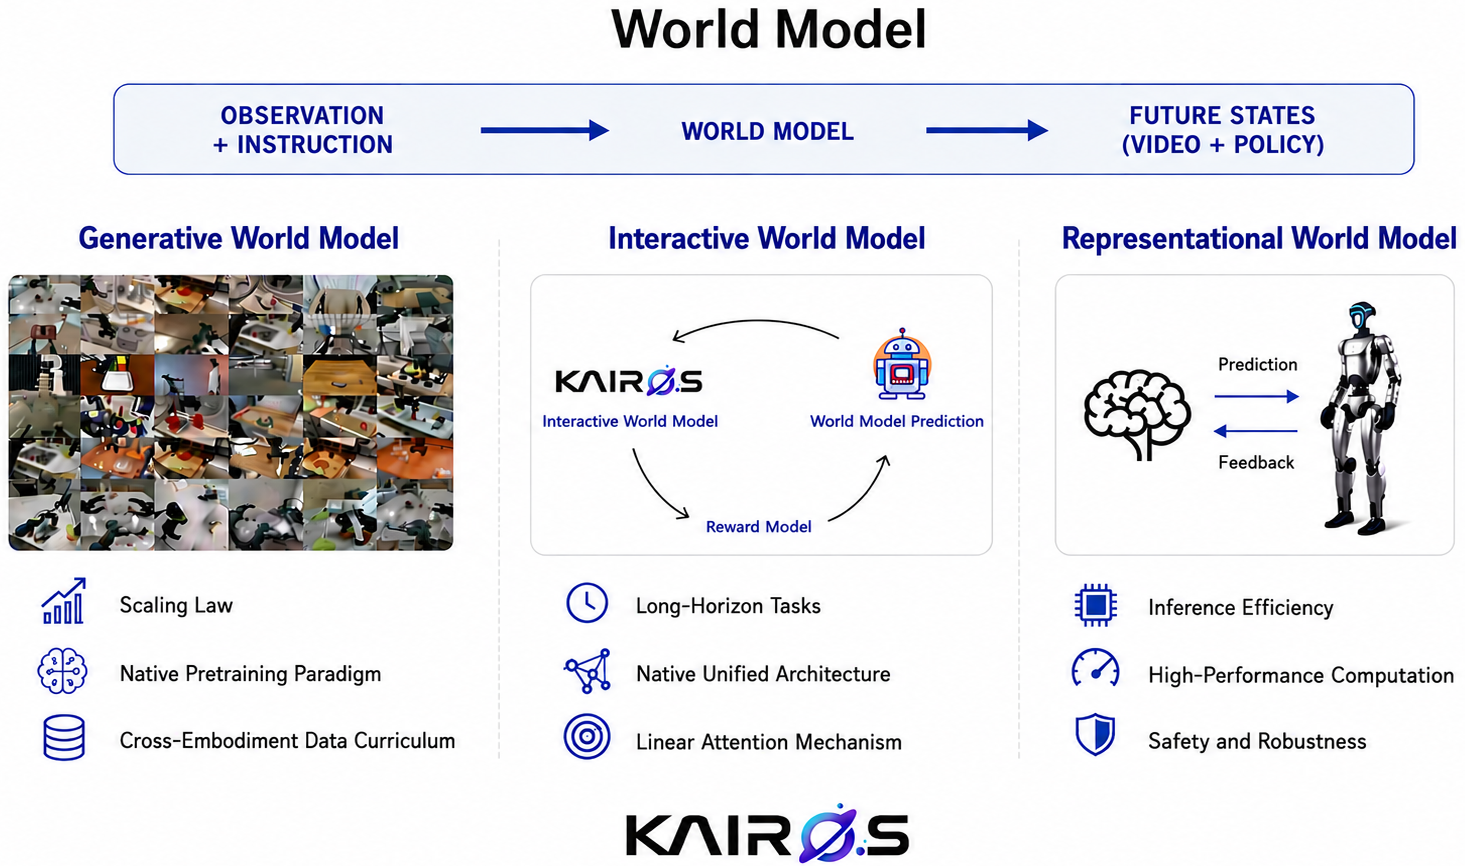
\includegraphics[width=1\linewidth]{figures/motivation_v1.png}
    \caption{Motivation of Kairos. It is not merely a generative model but a deployable infrastructure natively designed for future self-evolutionary learning in Physical AI.} 
    \label{fig:motivation}
\end{figure}


\begin{itemize}
\item The first major challenge is fragmented world learning across heterogeneous experience sources. The knowledge required for a capable world model is distributed unevenly across open-world videos, human behavioral traces, and scarce robot interaction data. Open-world videos offer broad physical and environmental regularities, but typically lacks action grounding and task intent. Human data reveals structured behavior and interaction patterns, but does not directly align with robot embodiment or control spaces. Robot data is the most relevant for embodied operation, yet remains expensive, narrow, and difficult to scale. As a result, current systems often optimize on one form of experience while underutilizing the others, learning partial competencies rather than unified world knowledge. This is difficult not merely because the datasets are large, but because the knowledge forms themselves are mismatched across perception, behavior, and embodiment. The consequence is substantial: models may learn broad physical priors without actionable grounding, or narrow robot skills without generalization, preventing them from serving as transferable substrates for embodied intelligence.

\item The second major challenge is maintaining persistent world states over long temporal horizons. Short video continuation can often rely on local visual smoothness, but world modeling requires something harder: preserving the same world over more time. This includes maintaining object permanence, delayed physical effects, multi-stage interactions, latent task progress, and causal consequences that may unfold only after substantial temporal gaps. Many current systems perform well on short-horizon appearance transitions yet degrade as duration grows, because local continuation heuristics do not guarantee global state consistency. As we formally prove in this report, this degradation is an unavoidable structural limitation. Purely local continuation heuristics are mathematically insufficient to guarantee global state consistency and inherently incur an irreducible excess risk. The difficulty is both representational and computational. Representationally, the model must retain the right abstract state variables rather than merely re-render recent observations. Computationally, dense temporal attention becomes increasingly prohibitive as duration and resolution grow, while simple autoregressive rollout accumulates drift and inconsistency. As a result, apparently strong long-video models may still fail as world models because they do not reliably preserve the world they are meant to simulate.

\item The third challenge is the gap between world understanding and embodied control. A model may predict or generate plausible futures, but fails to learn how actions from an embodied agent change those futures in a reliable, controllable way. This gap arises because observation, behavior, and control occupy different representational regimes: open-world videos rarely specify action-conditioned transitions, human demonstrations follow patterns that do not directly map to robot actuation, and robot interaction datasets are often too narrow to induce broad transferable priors. Consequently, many world models remain spectators of the world rather than participants in it. They may support visual forecasting or environment generation, yet still fail to provide stable perception-action grounding for downstream embodied decision-making. This limitation directly affects robotics and physical AI, where the central question is not just what will happen next, but what will happen if this agent acts now.

\item The fourth challenge is deployment and closed-loop operation under real-world constraints. Even a strong world model in offline evaluation may be unusable in practice if it cannot run with sufficiently low latency, low memory overhead, and realistic communication costs. This is not a peripheral engineering issue. For physical AI, and especially for any future form of self-evolution learning, the model must be able to participate in observation-action-feedback loops in real time or near real time. If inference is too slow, too memory-intensive, or too tightly tied to impractical hardware assumptions, the model cannot be embedded into real systems, cannot accumulate online corrective feedback, and cannot support continual embodied adaptation. In other words, without deployment-ready operation, world models remain demonstrations rather than infrastructure. This is why recent infrastructure-oriented efforts, such as Cosmos and Dreamer 4, place unusual emphasis on scalable operation and efficient inference rather than on model quality alone.
\end{itemize}



These challenges are tightly coupled. Fragmented learning makes it difficult to acquire coherent world knowledge; weak long-horizon state maintenance makes it difficult to preserve that knowledge over time; poor embodiment grounding makes it difficult to connect world knowledge to control; and the absence of deployment-ready execution prevents any of these capabilities from entering real observation–action–feedback loops. Addressing them separately risks producing systems that are strong along one dimension but fundamentally incomplete as substrates for physical intelligence.



Kairos is designed precisely around this bottleneck structure. Rather than treating these issues as separate engineering concerns, we address them jointly through a native world-action model stack that learns the world through progressive cross-embodiment experience, maintains the world through consistent temporal attention mechanism, and runs the world through deployment-aware system co-design. Besides, fundamentally departing from the prevalent yet disjointed practice of post-training or fine-tuning generic open-domain video generators for downstream embodied control, we pioneer a \textbf{Native Pre-training Paradigm for Physical AI}, championing the philosophy that general physical laws, behavioral semantics, and embodied grounding must be natively synthesized within the foundational architecture from the very inception of scaling, establishing a genuinely cohesive, deployment-aware world-action infrastructure. In this sense, Kairos is not only a stronger world model, but a step toward a world-model substrate that is operationally ready for future self-evolution learning in physical AI. 



\begin{figure}[t]
    \centering
    % 
\includegraphics[width=\linewidth]{kairos3.0//figures/framework.png}
 %   \includegraphics[width=\linewidth]{kairos3.0/figures/nartive_wm_architecture.pdf}
%    \includegraphics[width=\linewidth]{kairos3.0/figures/kairos_framework.jpg}
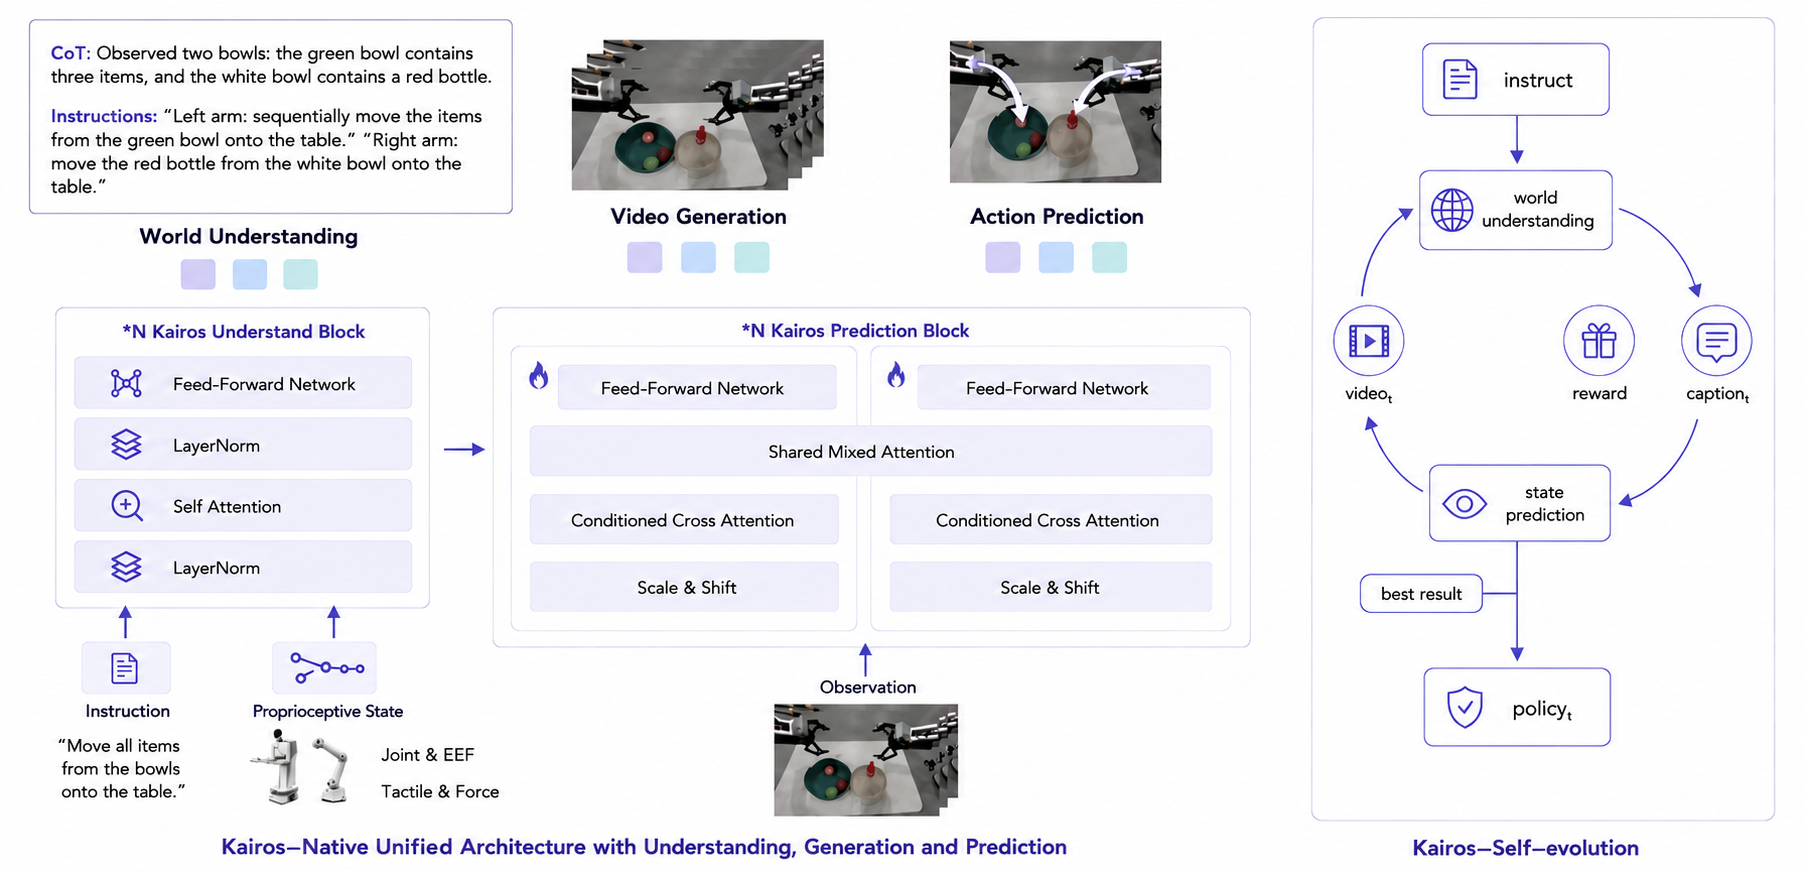
\includegraphics[width=1\linewidth]{figures/framework_new_v1.png}
    \caption{Framework of Kairos.}
    \label{fig:kairos_3_0_framework}
\end{figure}


\begin{figure}[tp]
    \centering


 % ---------- Lower group (2 images) ----------
    \begin{subfigure}{\linewidth}
        \centering
        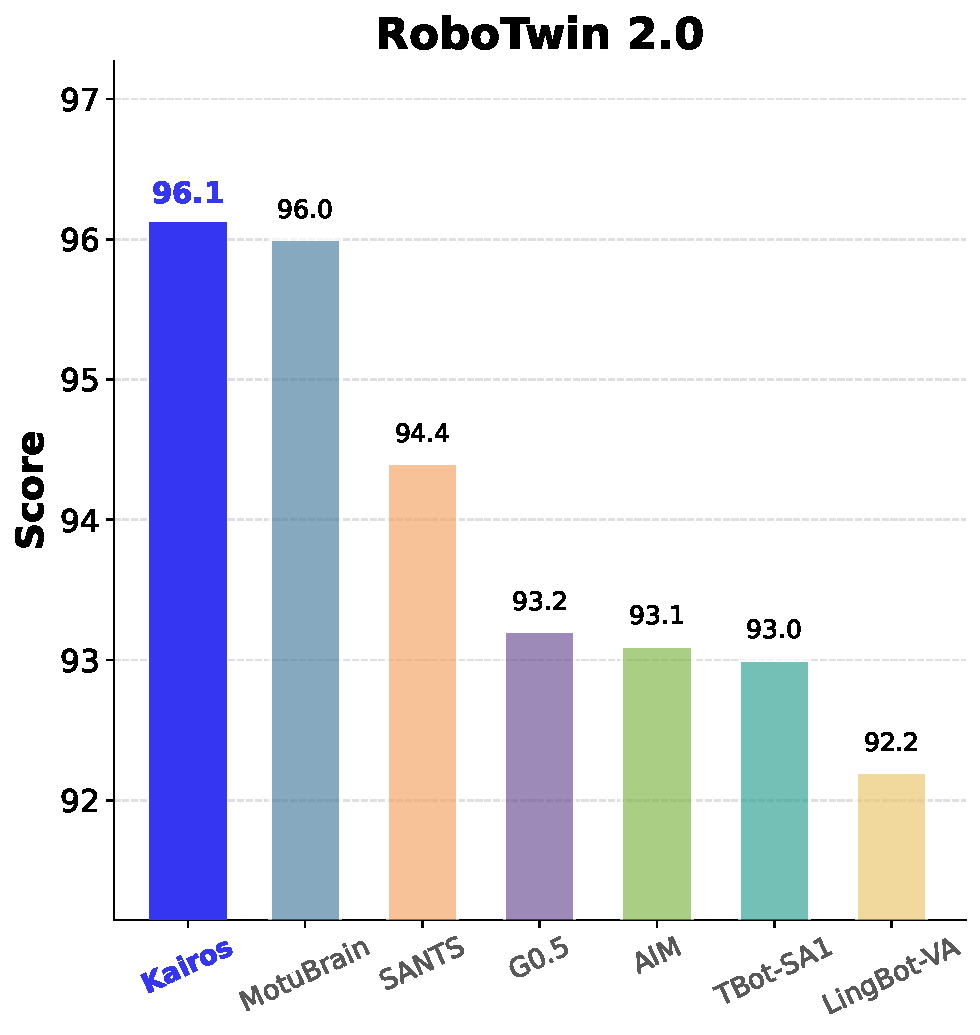
\includegraphics[width=0.4\linewidth]{figures/benchmark_robotwin_2.0.pdf}
       % \hfill
       \hspace{1em}
        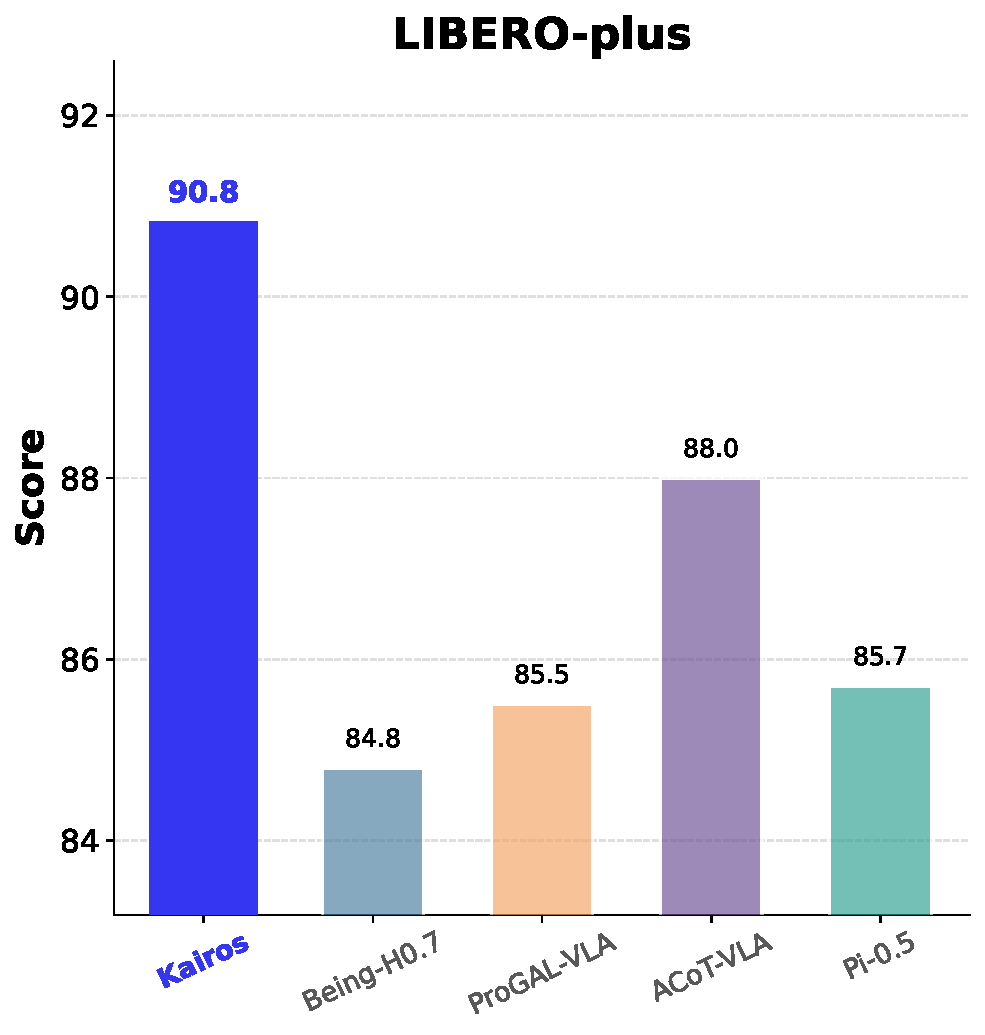
\includegraphics[width=0.4\linewidth]{figures/benchmark_libero-plus.pdf}
        \caption{Performance comparison across world action model benchmarks}
    \end{subfigure}

 \vspace{0.3em}
 
    % ---------- Upper group (3 images) ----------
    \begin{subfigure}{\linewidth}
        \centering
        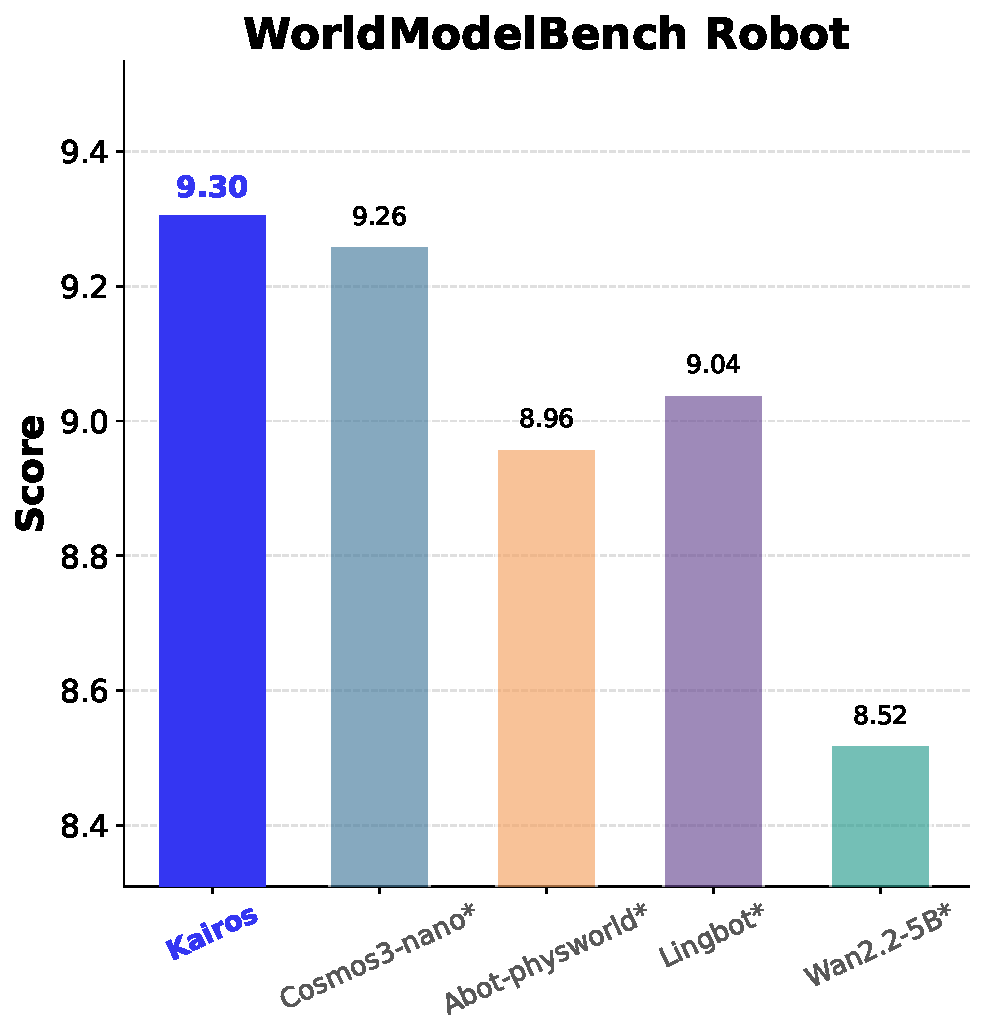
\includegraphics[height=0.4\linewidth]{figures/benchmark_worldmodelbench_robot.pdf}
       % \hfill
       \hspace{1em}
        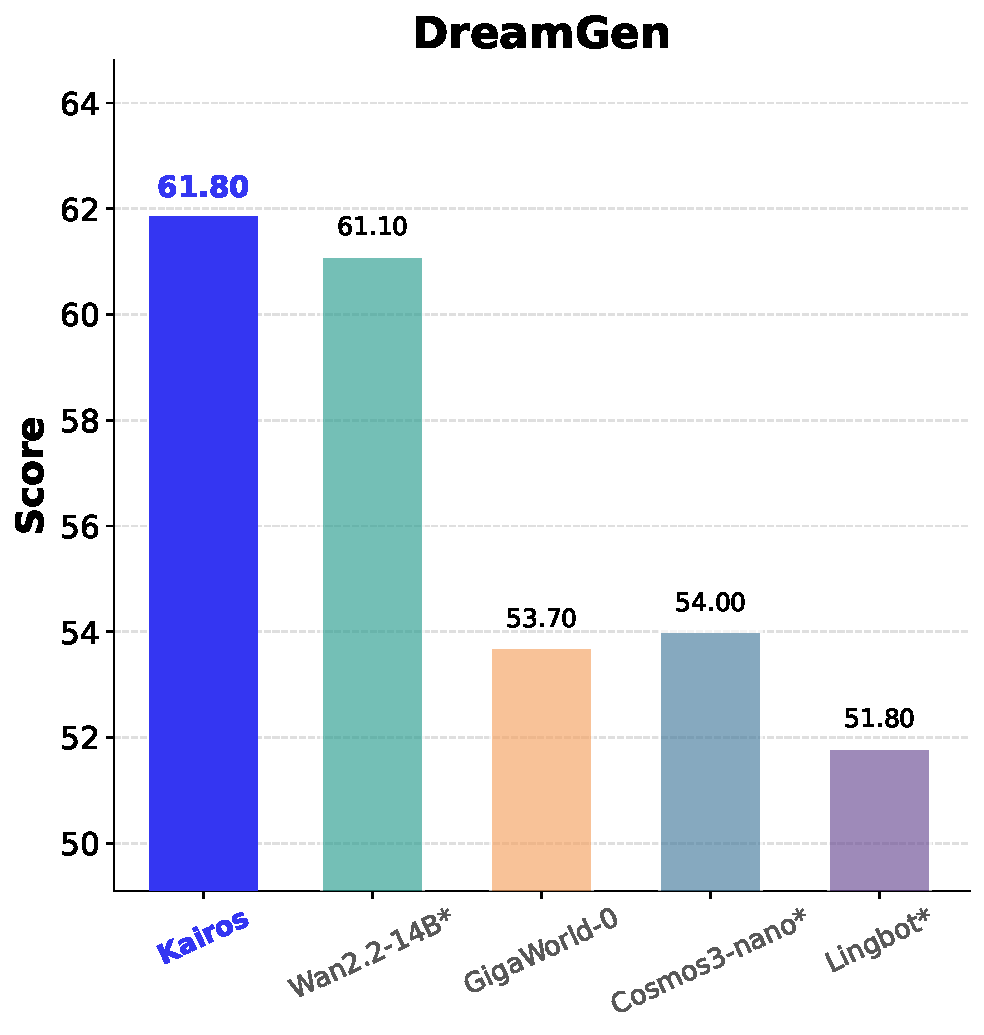
\includegraphics[height=0.4\linewidth]{figures/benchmark_dreamgen.pdf}
        \caption{Performance comparison across embodied world model benchmarks}
    \end{subfigure}

    \vspace{0.3em}

 

 
   % ---------- Lower group (2 images) ----------
    \begin{subfigure}{\linewidth}
        \centering
        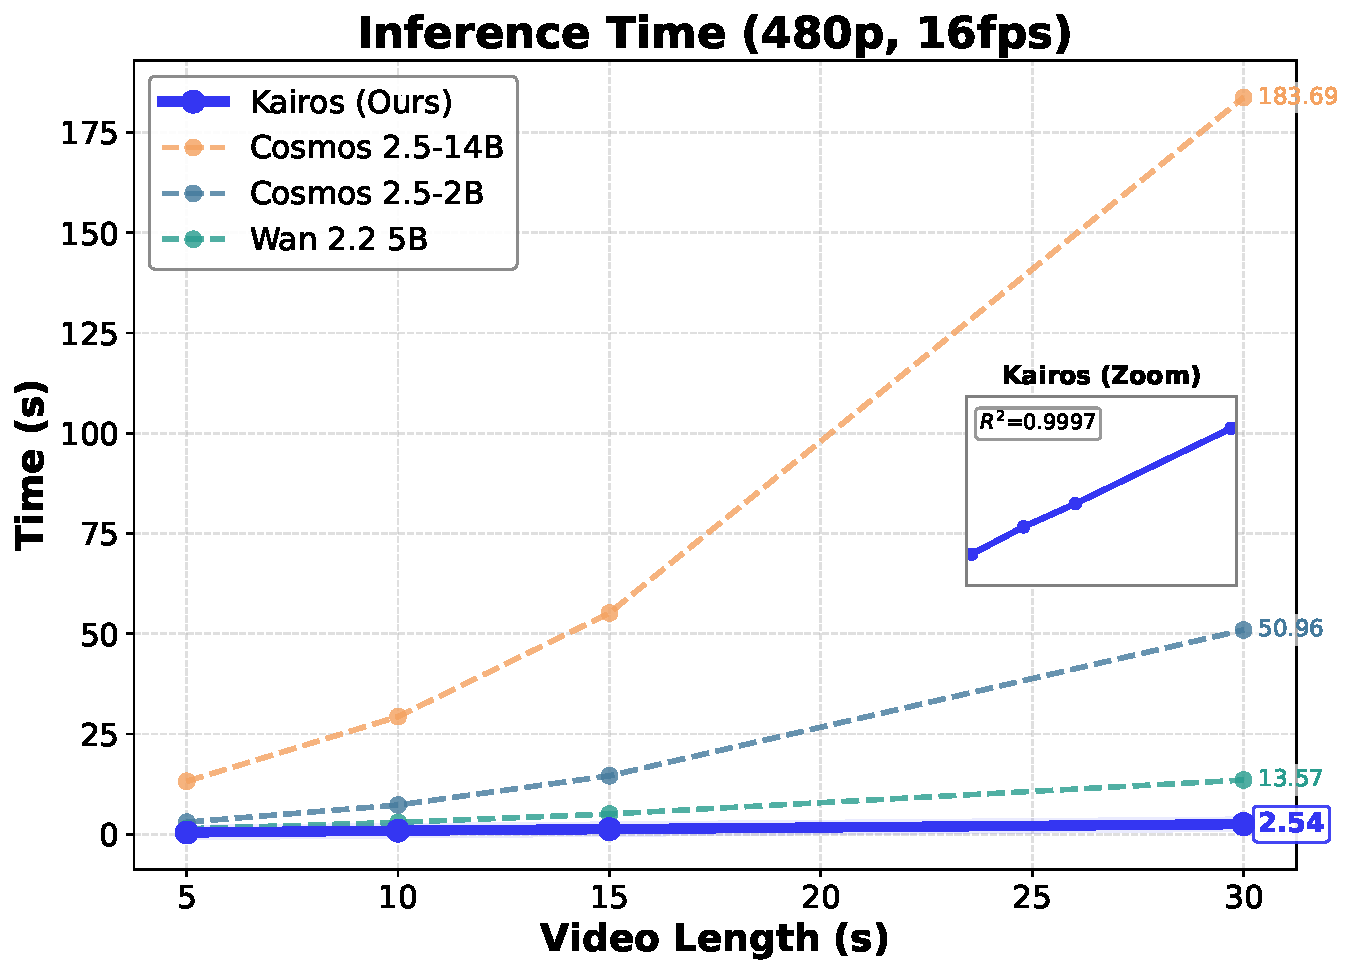
\includegraphics[width=0.49\linewidth]{figures/dit_inference_480p.pdf}
      %  \hfill
        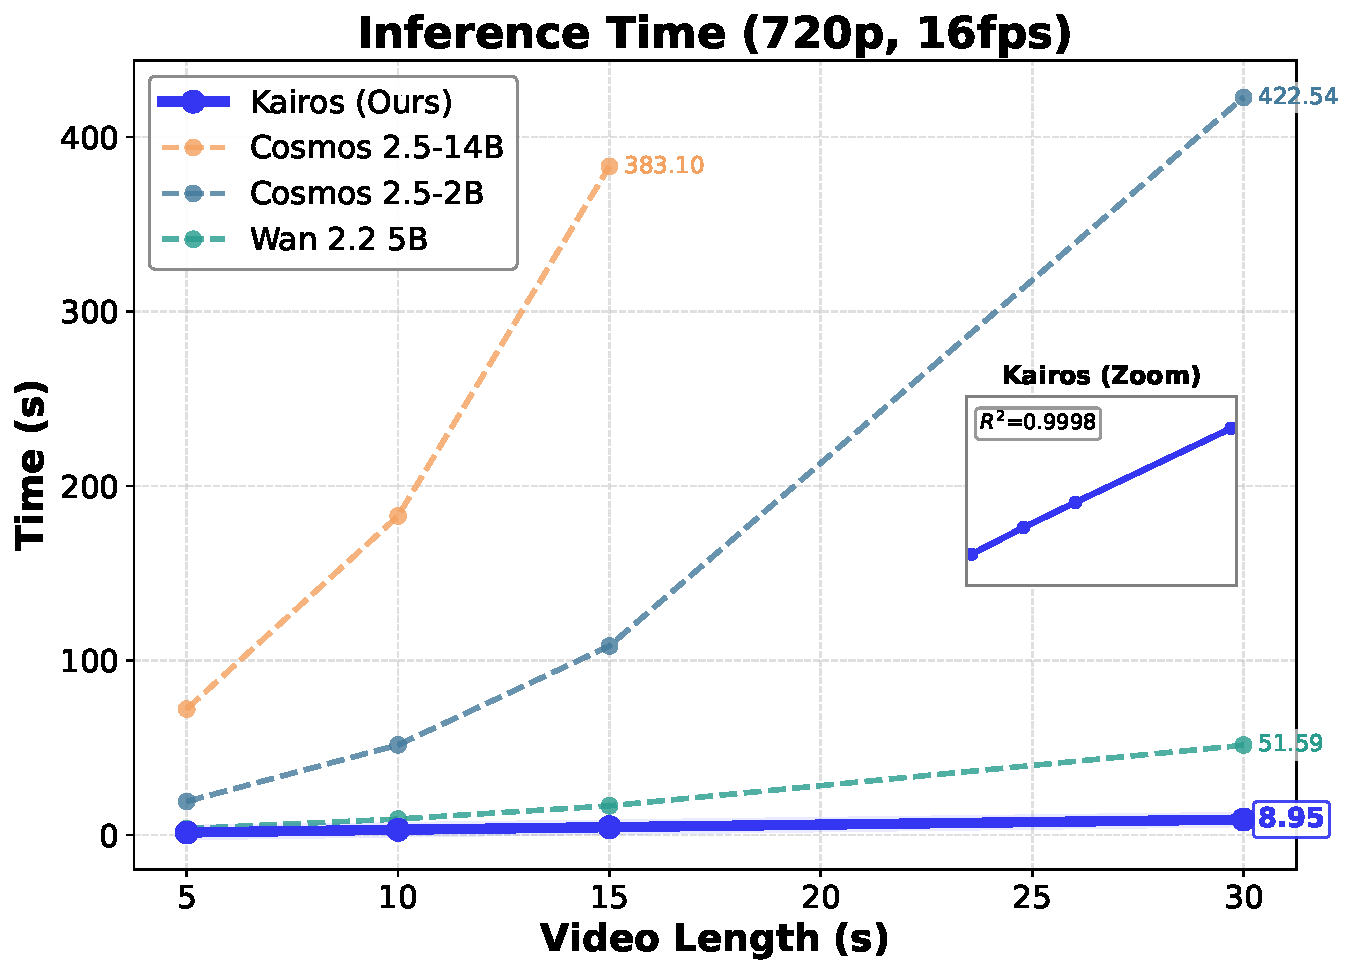
\includegraphics[width=0.49\linewidth]{figures/dit_inference_720p.pdf}
        \caption{Inference time comparison per DiT step}
    \end{subfigure}

    \caption{ (a) (b) Kairos achieves state-of-the-art performance across diverse both embodied world model and world action model benchmarks while delivering significant efficiency superiority over baseline models. (c) Notably, Kairos scales linearly (see the zoom window for the DiT inference time per step), ensuring consistent throughput for long-duration generation.}
    \label{fig:vs}
\end{figure}





The core contributions of this work are organized around three foundational echelons:

\begin{itemize}
    \item 
Our first contribution is the establishment of \textbf{A Native Pre-training Paradigm via Cross-Embodiment Data Curriculum (CEDC)}. We reject the decoupled post-training fine-tuning approach and instead propose a native pre-training paradigm that injects physical and behavioral knowledge from scratch. To operationalize this native injection across highly disparate data domains, self-evolution-inspired CEDC serves as the structural backbone of our pre-training phase, and organizes them into a progressive hierarchy. General videos provide broad physical and environmental regularities; human data contributes structured behavioral patterns and task organization; robot data grounds perception-action alignment and embodied control. Kairos moves beyond flat data scaling to propose a developmental world-knowledge curriculum. By organizing heterogeneous experience—from open-world observation to human imitation and robot embodiment—into a progressive hierarchy, the model systematically acquires internal representations that evolve from passive physics to active task-intent. 


\item Our second contribution is a \textbf{Native Understanding-Generation-Prediction Architecture with Hybrid Linear Temporal Memory}. Rather than framing long-horizon modeling as a pure video continuation problem, Kairos treats it as a persistent world-state task within a unified Mixture-of-Transformers (MoT) stack, where understanding supplies causal interpretation, generation unfolds physically plausible futures, and prediction outputs hardware-deployable action trajectories. To guarantee long-horizon state maintenance under linear computational complexity, we factorize temporal modeling via a hybrid attention mechanism: Sliding-Window Attention (SWA) anchors local dynamics, Dilated Sliding-Window Attention (DSWA) captures mid-range interactions, and Gated Linear Attention (GLA) serves as a contractive global causal memory. Crucially, we establish formal theoretical bounds demonstrating that this architectural factorization strictly limits error accumulation, mathematically guaranteeing persistent state propagation across extended horizons.

\item Our third contribution is a \textbf{Deployment-Aware System Co-Design} that treats real-time edge-side execution as a first-order modeling principle. We argue that for world models aspiring to future closed-loop self-evolution, systems optimization is not a post-hoc acceleration luxury, but an operational necessity. If inference latencies or memory footprints block the model from entering real observation–action–feedback loops, continual adaptation remains unattainable. By co-designing hardware-aware compute kernels, quantization protocols, and token streaming, Kairos sustains high-throughput, low-memory inference on consumer-grade hardware. This optimization establishes the definitive operational conditions under which real-world deployment and future self-evolutionary scaling can practically occur.





    
\end{itemize}















Crucially, these three pillars should not be read as isolated engineering additions, but as a deeply coupled response to the structural bottlenecks that prevent world models from becoming operational substrates for continuous \textbf{self-evolution}. Future physical agents cannot achieve autonomous self-evolution within static, decoupled frameworks. Kairos systematically resolves this by framing the world-modeling challenge around an evolvable capability chain that answers three fundamental questions: how to \textbf{learn}, \textbf{maintain}, and \textbf{run} worlds. 

First, the \textit{Cross-Embodiment Data Curriculum (CEDC)} defines how the model \textbf{learns} the world, mitigating the mismatch between broad ungrounded observations and narrow robotic actions. This structured data pyramid establishes a development-aligned progression—from passive physics to human behavior and active embodiment—providing a scalable knowledge pipeline for autonomous data collection and exploration. Second, the native understanding-generation-prediction stack equipped with hybrid linear temporal memory governs how the model \textbf{maintains} the world state. By strategically allocating temporal responsibilities across SWA (local dynamics), DSWA (mid-range interactions), and GLA (global contractive causal memory), the network robustly preserves critical world latents like object permanence over long horizons, mitigating the error accumulation that typically derails reinforcement learning rollouts. Third, the deployment-aware system co-design dictates how the model \textbf{runs} the world under real-world edge constraints. By optimizing low-level kernels and weight-only quantization, Kairos turns execution efficiency into a first-order modeling principle, enabling the sub-millisecond inference necessary to maintain the real-time observation–action–feedback loops through which self-evolution and online corrective learning practically occur.

\textbf{Results.} Extensive evaluations demonstrate that Kairos achieves state-of-the-art (SOTA) performance across diverse benchmarks while maintaining unprecedented inference efficiency (Figure \ref{fig:vs}). In general world-modeling and generative benchmarks as WorldModelBench \cite{li2025worldmodelbench} and DreamGen Bench \cite{fan2025dreamgen}, Kairos matches or surpasses significantly larger counterparts without incurring quadratic computational overhead, courtesy of its linear scalability. More importantly, when evaluated on rigorous embodied control and World-Action Model benchmarks, Kairos exhibits superior manipulation and generalization capabilities. It achieves new SOTA milestones on trajectory-driven task suites including LIBERO-plus and RoboTwin 2.0, firmly validating its efficacy as a deployable world-action execution infrastructure.

% --- Concluding Summary ---
%\textbf{Paradigm Shift in Physical AI.} 
Taken together, these architectural paradigms suggest a fundamental shift in how world models must be conceptualized. Rather than treating world modeling merely as a problem of rendering increasingly realistic pixels, Kairos treats it as the challenge of constructing a deployable, action-sensitive substrate that can acquire, preserve, and operationalize physical knowledge over time. By unifying a hierarchical curriculum, a hybrid persistent memory, and edge-side runtime co-design, Kairos moves beyond a static generative showcase, laying down the definitive operational foundation for future self-evolving physical intelligence.










